%%
%% 研究報告用スイッチ
%% [techrep]
%%
%% 欧文表記無しのスイッチ(etitle,eabstractは任意)
%% [noauthor]
%%

%\documentclass[submit,techrep]{ipsj}
\documentclass[submit,techrep,noauthor]{ipsj}

\usepackage[dvipdfmx]{graphicx}
\usepackage{latexsym}
\usepackage{booktabs}
\def\Underline{\setbox0\hbox\bgroup\let\\\endUnderline}
\def\endUnderline{\vphantom{y}\egroup\smash{\underline{\box0}}\\}
\def\|{\verb|}
%

%\setcounter{巻数}{59}%vol59=2018
%\setcounter{号数}{10}
%\setcounter{page}{1}


\begin{document}


\title{無順序木パターン言語の安定な生成に向けた\\表現設計とデータ拡張}

\etitle{Representation Design and Data Augmentation for Stable Generation of Unordered Tree Pattern Languages}

\affiliate{FIT-grad}{福岡工業大学大学院工学研究科\\
Department of Information Engineering, Fukuoka Institute of Technology,3-30-1, Washirohigashi, Higashi-ku, Fukuoka City, Fukuoka Prefecture, 811-0295, Japan}


\affiliate{FIT}{福岡工業大学情報工学部, Faculty of Information Engineering, Fukuoka Institute of Technology}
\affiliate{HCU}{広島市立大学大学院情報科学研究科, Graduate School of Information Sciences, Hiroshima City University}
\affiliate{TU}{東海大学理学部, School of Science, Tokai University}

\author{稗田 桃子}{Momoko Hieda}{FIT-grad}[mfm25110@bene.fit.ac.jp]
\author{正代 隆義}{Takayoshi Shoudai}{FIT}[shodai@fit.ac.jp]
\author{内田 智之}{Tomoyuki Uchida}{HCU}[uchida@hiroshima-cu.ac.jp]
\author{松本 哲志}{Satoshi Matsumoto}{TU}[matsumoto@tokai-u.ac.jp]
\author{鈴木 祐介}{Yusuke Suzuki}{HCU}[y-suzuki@hiroshima-cu.ac.jp]

\begin{abstract}
本研究では，葉に構造的変数をもつラベル付き無順序木パターンが定める木言語を対象とし，
その正例集合から深層生成器を学習する問題を扱う．
無順序木を学習入力へ変換する際，同一の木構造であっても兄弟ノードの順序の違いにより
頂点 ID 表現が変動する（表現ゆらぎ）．
この現象は生成器の学習安定性を損なう要因となり，
特に難しいパターンでは seed によって生成性能が大きく低下する場合がある．
本研究では，兄弟順序のランダム化に基づくデータ拡張を導入し，
表現ゆらぎを緩和することで学習の安定化を図る．
7 条件・10 seed の計 70 件の実験において，
経験的潜在分布からの生成性能（empirical\_latent）はすべての条件で 0.89 以上となり，
極端な失敗例は観測されなかった．
これにより，表現ゆらぎを考慮した学習法が
無順序木パターン言語の安定な深層生成に有効であることを示す．
\end{abstract}

\begin{jkeyword}
無順序木パターン，深層生成モデル，VAE-GAN，表現ゆらぎ，データ拡張，潜在空間生成
\end{jkeyword}

\begin{eabstract}
This paper addresses the problem of learning a deep generative model
for the language defined by a labeled unordered tree pattern with structural variables.
When converting unordered trees into graph representations for neural network input,
the vertex ID assignment varies depending on the sibling order,
even for structurally equivalent trees.
We refer to this phenomenon as \textit{representation fluctuation},
which can destabilize training and cause significant performance degradation
for certain random seeds, especially on hard patterns.
To address this issue, we introduce a data augmentation method
based on sibling order randomization combined with BFS renumbering,
aiming to reduce the dependence on specific vertex ID assignments.
Experiments over 70 runs (7 configurations $\times$ 10 seeds) show that
the empirical-latent match rate remains at or above 0.89 across all conditions,
with no catastrophic failures observed.
These results demonstrate the effectiveness of the proposed approach
in achieving stable generation of unordered tree pattern languages.
\end{eabstract}

\begin{ekeyword}
unordered tree pattern, deep generative model, VAE-GAN,
representation fluctuation, data augmentation, empirical latent generation
\end{ekeyword}

\maketitle


\section{はじめに}

無順序ラベル付き木パターンは，木構造データの集合を表現するための自然な枠組みであり，XML 文書処理や生命情報科学などを背景とする構造データのモデル化に広く関係している．このようなパターンが定める正例集合を学習し，その言語を近似的に生成できるモデルを構築することは，知識獲得や構造的データの理解において重要な問題である．

しかし，無順序木を深層生成モデルへ入力するためには，BFS 順に基づく再番号付けを経てグラフ表現へ変換する必要がある．このとき，同一の木構造であっても兄弟ノードの順序の違いにより頂点 ID が変動し，等価な木が異なる表現として与えられる現象（表現ゆらぎ）が生じる．特に，浅い変数に大きな部分木が代入されるパターンでは，この変動が顕著になり，seed によっては学習が不安定になる場合があることが予備的実験により確認されている．

本稿では，この表現ゆらぎに対処するため，child\_origin 表現の採用，兄弟順序のランダム化に基づくデータ拡張，および Empirical Latent 生成戦略を組み合わせた生成パイプラインを提案する．実験では，7 条件・10 seed の計 70 件において empirical\_latent が 0.89 以上であり，極端な失敗例は観測されなかった．この結果は，提案法が表現ゆらぎの影響を緩和し，複数 seed に対して安定した生成を実現できることを示している．

以下，2章では関連研究を述べ，3章で提案法を説明する．4章で実験設定，5章で実験結果，6章で考察を示し，7章でまとめる．

\section{関連研究・背景}

\subsection{無順序木パターンマイニング}

無順序ラベル付き木を対象とするパターンマイニングは，XML 文書処理や生命情報科学などを背景として広く研究されてきた．Zaki~\cite{zaki2005} は埋め込み無順序部分木を対象とした頻出パターンマイニングアルゴリズム SLEUTH を提案し，Chehreghani ら~\cite{chehreghani2007} は最大埋め込み無順序木をトップダウンに探索する手法 TDU を示している．これらの研究は，大規模な木データベースから頻出する部分構造を効率よく列挙・抽出することを主目的としている．

これに対して，本研究の目的は，既知の無順序木パターンが生成する正例集合を学習し，その言語を近似的に生成可能なモデルを構成することにある．したがって，本研究は頻出パターンの列挙そのものではなく，無順序木パターン言語の学習と生成を対象としている点で，従来のパターンマイニング研究とは問題設定を異にする．

\subsection{グラフ・木の深層生成モデル}

グラフ生成に対する深層学習の応用として，GraphVAE~\cite{simonovsky2018} は隣接行列を変分オートエンコーダによりモデル化する枠組みを提案し，JT-VAE~\cite{jin2018} は分子グラフを Junction Tree を介して生成する手法を示している．また，木構造や木分解を利用した生成手法として，TD-GEN~\cite{shirzad2022} なども提案されている．これらの研究は，一般グラフや分子グラフの生成を主対象としており，深層生成モデルの有効性を示してきた．

一方で，本研究が対象とするのは，単一のグラフや木を生成する問題ではなく，ある無順序木パターンが定める言語に属する正例集合を学習対象とし，その分布を近似的に生成する問題である．さらに，本研究では生成性能そのものに加えて，学習の安定性，とくに初期値や seed に対する頑健性に着目している．このような観点は，一般的なグラフ生成研究では必ずしも中心的に扱われてきたわけではなく，本研究の特徴の一つである．

\subsection{グラフニューラルネットワークと関係型畳み込み}

グラフ構造を直接扱う深層学習手法として，Kipf ら~\cite{kipf2017} による GCN や，Hamilton ら~\cite{hamilton2017} による GraphSAGE などが提案されている．これらはグラフ上の局所構造を集約することで，ノードやグラフ全体の表現学習を可能にするものであり，現在ではグラフ学習の基本的な枠組みとなっている．

本研究では，無順序木に付与されたエッジラベルを明示的に扱う必要があるため，Schlichtkrull ら~\cite{schlichtkrull2018} による関係型グラフ畳み込み（RGCNConv）をエンコーダに採用する．RGCNConv は，各エッジ種別を関係として扱い，多関係グラフ上での表現学習を可能にする．この性質により，無順序木におけるラベル付き辺を自然にモデルへ組み込むことができる．したがって，本研究における RGCNConv の採用は，木構造そのものだけでなく，ラベル付き関係構造としての無順序木を表現するうえで重要である．

\subsection{データ拡張と表現の安定化}

深層学習において，入力表現のわずかな変動が学習結果に影響を与えることは広く知られており，画像認識~\cite{shorten2019} や自然言語処理~\cite{wei2019} においては，データ拡張が表現の安定化や汎化性能向上に有効であることが示されている．これらの考え方は，構造データに対しても一定程度適用可能である．

本研究で扱う無順序木では，本来，兄弟ノードの順序は本質的な意味を持たない．しかし，実装上は BFS に基づく再番号付けや頂点 ID の付与を通じて，等価な木構造であっても入力表現が変動しうる．このような表現ゆらぎは，学習の不安定化や seed 依存性の一因となる可能性がある．少なくとも著者らの知る限り，無順序木パターン生成の文脈において，この種の BFS 再番号付け由来の表現変動を主題化し，その影響を系統的に検討した研究は限られている．

そこで本研究では，兄弟順序のランダム化と再番号付けを組み合わせたデータ拡張を導入し，この表現ゆらぎを緩和することで，生成性能および学習安定性の改善を目指す．

\section{提案法}

\subsection{問題設定}

本研究では，葉の一部に変数をもつ根付きラベル付き無順序木を無順序木パターンと呼ぶ．ここで変数とは，任意の無順序木で置換可能な特別な葉である．無順序木 T がパターン P にマッチするとは，P の各変数に無順序木を代入することにより T が得られることを意味する．P にマッチする木全体の集合を P の正例集合と呼ぶ．
本研究の目的は，ある無順序木パターン P の正例集合から深層生成モデルを学習し，P の言語を近似的に生成できるモデルを構築することである．なお，生成された木集合を下流の推論アルゴリズムへ入力した場合の挙動については，補足的に確認する．

\subsection{入力表現と表現ゆらぎ}

無順序木はそのままではニューラルネットワークへの入力に適さないため，本研究では正例木を BFS 順に再番号付けしたグラフ表現へ変換する．しかし，同一の無順序木であっても，兄弟ノードの並び方が異なると BFS による頂点番号付けが変化し，結果として入力表現も変動する．本稿ではこの現象を表現ゆらぎと呼ぶ．

この表現ゆらぎは，本来等価である木構造に対して異なる入力表現を与えるため，エンコーダがそれらを異なる潜在表現として扱う原因となりうる．特に，浅い位置の変数へ大きな部分木が代入される場合には，頂点 ID の変動が大きくなりやすく，学習の不安定化を招く可能性がある．本研究では，この表現ゆらぎが生成性能や seed 依存性に与える影響に着目する．

\subsection{child\_origin 表現}

本研究では，ノード特徴量として child\_origin 表現を採用する．これは，各ノードが「どの親ノードから到達したか」と「その親子間のエッジラベル」を child 側の特徴として保持する表現である．この表現により，無順序木における親子関係とラベル情報を明示的にモデルへ与えることができる．

child\_origin 表現は，隣接構造全体を一様に扱う方法に比べて，無順序木における局所的な親子関係を自然に反映できる．また，番号付けそのものよりも親子関係とラベルを重視するため，表現ゆらぎの影響を相対的に抑えることが期待される．

\subsection{VAE-GAN アーキテクチャ}

\begin{figure*}[t]
\begin{center}
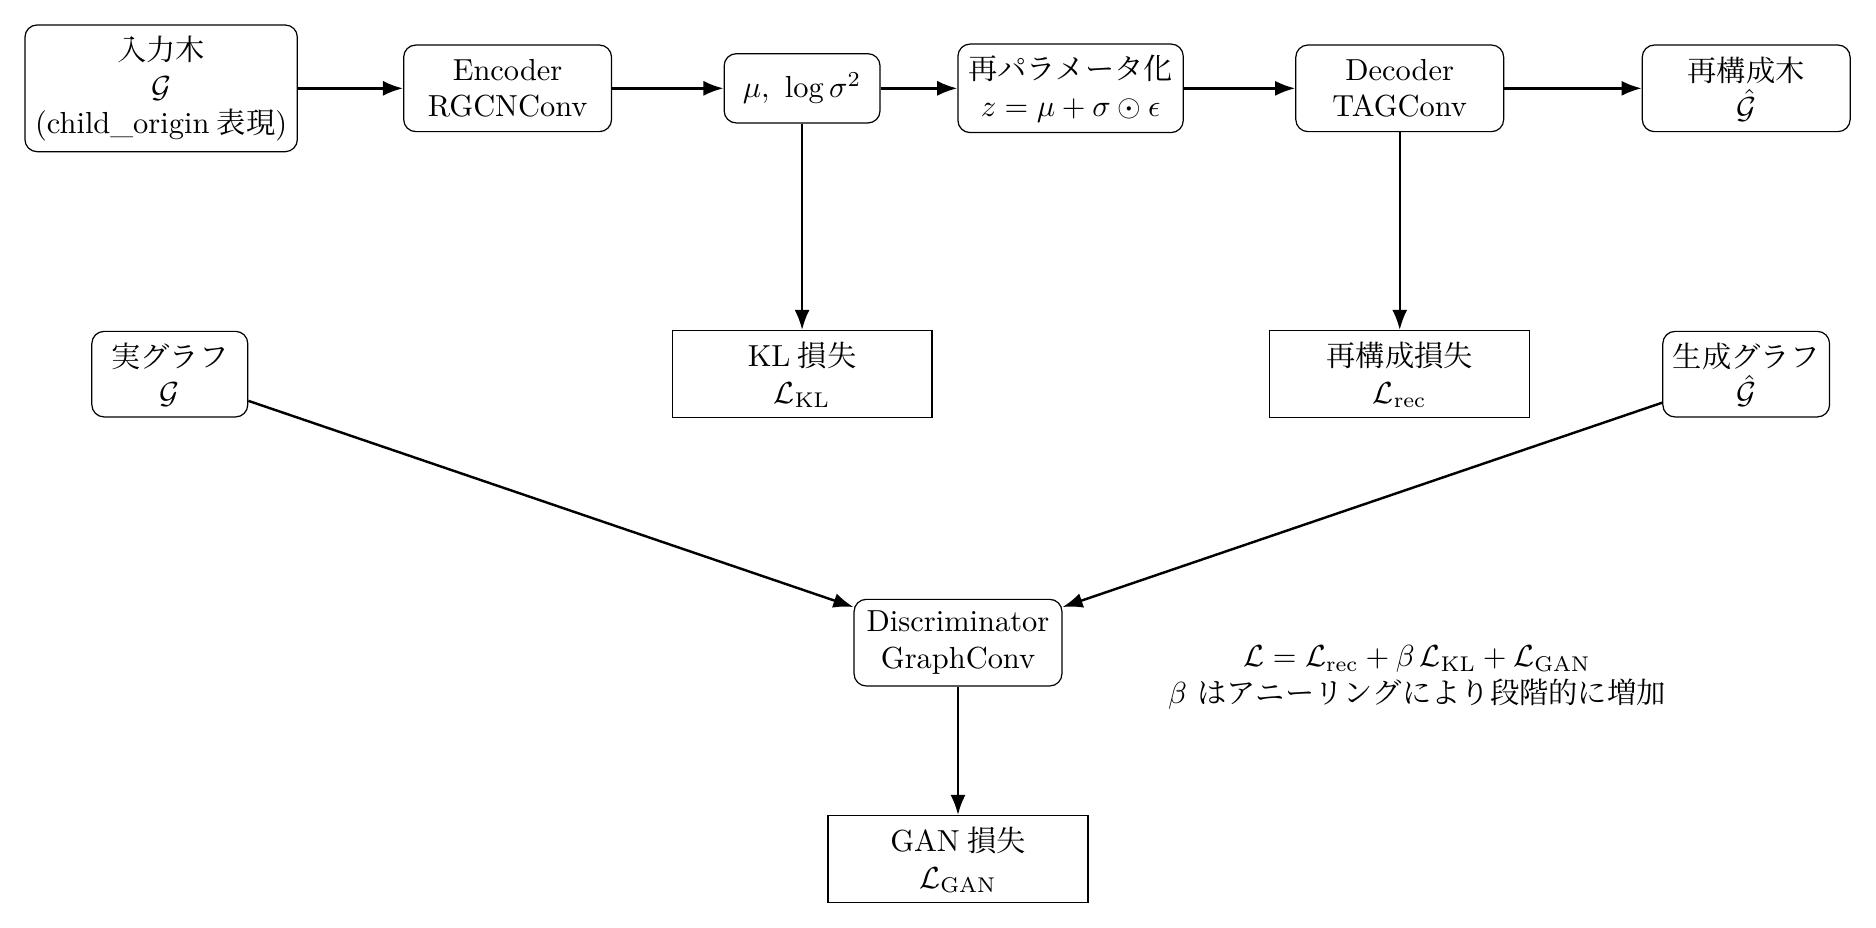
\includegraphics[width=0.8\linewidth]{vae-gan-architecture-clean.jpeg}
\end{center}
\caption{提案する VAE-GAN アーキテクチャの概略図．入力木を child\_origin 表現に変換し，Encoder（RGCNConv）で潜在表現へ写像する．再パラメータ化により得た潜在変数 $z$ を Decoder（TAGConv）へ入力し，再構成木を生成する．Discriminator には GraphConv を用い，実グラフと生成グラフの識別を行う．学習では，再構成損失，KL 損失，GAN 損失を組み合わせ，$\beta$ を段階的に増加させる．}
\label{fig:vae-gan-architecture}
\end{figure*}

提案モデルは Encoder，Decoder，Discriminator から構成される VAE-GAN 型の生成器である（図\ref{fig:vae-gan-architecture}）．Encoder には関係型グラフ畳み込み RGCNConv を採用する．RGCNConv はエッジの種類ごとに異なる重み行列を学習するため，無順序木に付与されたラベル付きエッジを多関係構造として明示的に扱うことができる．Encoder は各ノードの潜在表現を出力し，再パラメータ化トリックにより潜在ベクトルをサンプリングする．

Decoder には TAGConv を採用する．TAGConv は複数ホップ近傍の情報を集約できるため，木構造の局所的接続関係を再構成するのに適している．一方，Discriminator には GraphConv を採用する．GraphConv は近傍情報の集約を通じて局所的な接続密度や次数の影響を反映しやすく，生成グラフと実グラフの構造差を識別するのに有効である．本研究では，Discriminator においてこの性質を利用し，次数の影響力を高めることで識別性能の向上を図る．

学習では，再構成損失，KL 損失，GAN 損失を組み合わせた目的関数を用いる．さらに，β-VAE 的なアニーリングにより KL 項の重みを段階的に増加させ，潜在空間の安定化と再構成性能の両立を図る．

\subsection{データ拡張による表現ゆらぎの緩和}

表現ゆらぎに対処するため，本研究では兄弟順序のランダム化と BFS 再番号付けを組み合わせたデータ拡張を導入する．具体的には，各正例木に対して兄弟ノードの順序をランダムに並べ替えたうえで再番号付けを行い，同一の木から複数の表現を生成して学習データへ追加する．

この拡張により，モデルが特定の BFS 番号付けパターンに過適合することを防ぎ，本来等価な無順序木を近い潜在表現として学習しやすくなると期待される．したがって，本研究ではデータ拡張を，単なるデータ数増加ではなく，表現ゆらぎの緩和による学習安定化手法として位置づける．

\subsection{Empirical Latent 生成}

学習済みモデルからの生成には，Empirical Latent 生成を用いる．これは，正例木から得られた潜在表現をバンクとして保持し，その中から代表点を選択したうえで，その近傍にノイズを加えてサンプリングする方式である．代表点の選択には Farthest Point Sampling（FPS）またはランダム選択を用い，ノイズの強さは別途制御する．

この方式の狙いは，訓練データの潜在分布から過度に離れた点を直接サンプリングするのではなく，観測された潜在表現の近傍を利用して，正例言語により忠実な生成を行うことである．その結果，潜在空間全体を一様に探索する場合に比べて，生成の安定性と妥当性の向上が期待される．

\subsection{パイプライン全体}

提案パイプラインは次の 4 段階からなる。
\begin{enumerate}
\item 学習段階：正例木集合から VAE-GAN を学習する
\item 評価段階：潜在表現に基づく再生成や Empirical Latent 生成により，生成品質を評価する
\item 生成段階：学習済みモデルを用いて新規木集合を生成する
\item 推論段階：生成木集合を下流の推論アルゴリズムへ入力し，推定パターン P' を得る
\end{enumerate}

本研究では，生成器単体の性能だけでなく，生成結果が下流推論に与える影響も補足的に確認する．この意味で，本研究の対象は単なる木生成ではなく，生成から推論までを含む一連の知識獲得過程である．

\section{実験設定}

\subsection{実験目的}

本実験の目的は，提案した入力表現，データ拡張，および生成戦略が，無順序木パターン言語の生成品質と学習安定性にどのような影響を与えるかを評価することである．特に，乱数 seed の違いによる性能変動に着目し，hard seed を含む複数条件において安定した生成が可能かを検証する．また，生成された木集合を下流の推論アルゴリズムへ入力した場合に，推定パターン P' がどの程度妥当なものとなるかも補足的に確認する．

\subsection{データ生成条件}

実験では，ラベル付き無順序木パターンから生成した正例木集合を学習対象とする．主な設定は，パターン頂点数，追加頂点数，辺ラベル数，および正例数である．本研究では，辺ラベル数を 5，パターン頂点数を 10，追加頂点数を 10 とした．正例数については，データ量依存性を調べるため，主に 500，1000，2000 を用いた．

\subsection{モデルおよび学習条件}

提案モデルは，Encoder，Decoder，Discriminator からなる VAE-GAN 型構成を採用する．Encoder には RGCNConv，Decoder には TAGConv，Discriminator には GraphConv を用いた．学習時の主な設定は，近傍集約の次数 K，KL 項の最大重み，学習エポック数，およびエンコーダ層数である．また，KL 項については β-VAE 的なアニーリングを導入し，学習初期から一様に強い正則化を課すのではなく，段階的に重みを増加させることで学習の安定化を図った．

\subsection{生成条件}

学習済みモデルからの生成には，Empirical Latent 生成戦略を用いた．主な設定は，潜在バンクサイズ，代表点の選択方法，およびノイズスケールである．代表点選択には主に Farthest Point Sampling を用いた．標準設定としてはバンクサイズ 100 を中心に用い，比較のため full および 20 も評価した．なお，実際に利用可能な潜在表現数が設定したバンクサイズより少ない場合には，利用可能な個数に応じて実効的なバンクサイズが決まる．

\subsection{データ拡張条件}

表現ゆらぎを緩和するため，兄弟順序のランダム化と BFS 再番号付けを組み合わせたデータ拡張を導入した．各正例木に対して追加するランダム化表現の個数を拡張回数として制御し，本研究では拡張なしと拡張ありを比較した．拡張は学習データに対してのみ適用し，評価・生成時には用いていない．

\subsection{評価指標}

生成品質の評価には，主に encoded\_z と empirical\_latent を用いた．encoded\_z は，テストデータをエンコードした潜在表現に基づいて再生成した木が，元のパターン言語に属する割合を表す．empirical\_latent は，Empirical Latent 生成により得られた木集合のうち，元のパターン言語に属する割合を表す．

さらに，生成された木集合の多様性をみるために，異なる非同型木の個数を記録した．生成結果全体の妥当性については，blind 生成された木集合を元のパターン P に対して照合し，正例となる木の割合を生成マッチ率として評価した．下流推論については補足的に，推定パターン P' と元パターン P の差分として，ノード数差，辺数差，変数数差，DFUDS 長差，特化度，および P' の元正例集合に対するマッチ率を記録した．

\subsection{比較設定}

実験では，主として次の 3 系列の比較を行った．第 1 に，データ量依存性を確認するため，正例数を 500，1000，2000 と変化させた比較を行った．第 2 に，潜在バンクサイズの影響を調べるため，正例数を 1000 に固定して full，100，20 を比較した．第 3 に，データ拡張の効果を確認するため，正例数を 1000 に固定して拡張なしと拡張ありを比較した．各条件について複数の seed で実験を行い，seed に対する頑健性も評価した．

\subsection{実行環境と結果記録}

実験は Ubuntu 環境上で実施した．各 run では，学習，評価，生成，推論の各段階を順に実行し，結果を実験ディレクトリに保存した．各ディレクトリには設定ファイル，各段階のログ，生成木集合，推論後パターン評価，および各種指標をまとめた要約ファイルが残される．最終的には，複数 run の要約情報を 1 実験 1 行の表に集約し，seed，設定条件，生成性能，blind 生成の妥当性，および P と P' の差分を横断的に比較した．

\section{実験結果}

\subsection{生成性能の評価}

\begin{table*}[t]
\centering
\small
\caption{各設定における empirical\_latent の結果}
\label{tab:empirical-latent}
\begin{tabular}{lccccc}
\toprule
設定 & 正例数 & 拡張回数 & 最小値 & 最大値 & 平均値 \\
\midrule
np500\_bank100       & 500  & 1 & 0.930 & 1.000 & 0.988 \\
np1000\_bank100      & 1000 & 1 & 0.980 & 1.000 & 0.998 \\
np2000\_bank100      & 2000 & 1 & 0.990 & 1.000 & 0.999 \\
np1000\_bankfull     & 1000 & 1 & 0.920 & 1.000 & 0.985 \\
np1000\_bank20       & 1000 & 1 & 0.980 & 1.000 & 0.998 \\
np1000\_aug0\_bank100 & 1000 & 0 & 0.890 & 1.000 & 0.981 \\
np1000\_aug1\_bank100 & 1000 & 1 & 0.920 & 1.000 & 0.985 \\
\bottomrule
\end{tabular}
\end{table*}

\begin{table}[t]
\centering
\small
\caption{各設定群における生成木の多様性（unique\_graphs）}
\label{tab:unique-graphs}
\begin{tabular}{lccc}
\toprule
設定群 & 最小値 & 最大値 & 平均値 \\
\midrule
bank100 系（5設定） & 100 & 100 & 100.0 \\
bank20              & 20  & 62  & 28.6 \\
bankfull            & 100 & 100 & 100.0 \\
\bottomrule
\end{tabular}
\end{table}

\begin{table*}[t]
\centering
\small
\caption{代表的設定における推定パターン $P'$ と元パターン $P$ の差分}
\label{tab:pattern-diff}
\begin{tabular}{lccccc}
\toprule
設定 & $\Delta$ノード数 & $\Delta$辺数 & $\Delta$変数数 & $\Delta$DFUDS長 & $P'$ のマッチ率 \\
\midrule
np1000\_aug0\_bank100（seed=1241） & $-4$ & $-4$ & $-1$ & $-16$ & 1.00 \\
np1000\_aug1\_bank100（seed=1241） & $-1$ & $-1$ & $0$  & $-4$  & 1.00 \\
np1000\_bank100（seed=1234）       & $+1$ & $+1$ & $+1$ & $+4$  & 1.00 \\
\bottomrule
\end{tabular}
\end{table*}

表\ref{tab:empirical-latent}に，各設定・各 seed における encoded\_z および empirical\_latent の値を示す．
全70件（7設定 × 10 seed）において，empirical\_latent は 0.89 以上であり，0.7 を下回るケースは観測されなかった．正例数を増加させることで安定性が向上する傾向が見られ，正例数 1000 および 2000 の条件では最小値がそれぞれ 0.98，0.99 に達した．

データ拡張の効果については，拡張なし（augment=0）と拡張あり（augment=1）の比較から，次の傾向が確認された．拡張なしでは empirical\_latent の平均 0.981，最小値 0.89 であったのに対し，拡張ありでは平均 0.985，最小値 0.92 であった．特に，条件内で最も低い性能を示した seed において，拡張なしの 0.89 から拡張ありの 0.92 への改善が見られた．この結果は，データ拡張が表現ゆらぎの緩和を通じて最悪ケースの性能を底上げする効果をもつことを示唆する．

潜在バンクサイズについては，比較した設定の中では bank=100 が性能と多様性のバランスのよい結果を示した．以上より，Empirical Latent 生成は複数 seed に対して安定した生成性能を示し，特に bank=100 は標準設定として有望である．

\subsection{生成木の妥当性と多様性評価}

表\ref{tab:unique-graphs}に，blind 生成における生成マッチ率および非同型グラフ数の結果を示す．
全条件において生成マッチ率は高い水準を維持しており，生成された木の大部分が元のパターン言語に属することが確認された．一方，多様性については，bank=100 が bank=20 に比べて多くの非同型木を生成できることが示された．これは，バンクサイズが大きいほど潜在空間の広い範囲をカバーできるためと考えられる．bank=20 は高い妥当性を示す一方で多様性が低下する傾向が見られたため，妥当性と多様性の両面を考慮すると，bank=100 が標準設定の候補として妥当である．

\subsection{下流推論結果の確認}

表\ref{tab:pattern-diff} に代表的な設定における $P'$ と $P$ の差分を示す．
最悪ケースであった np1000\_aug0\_bank100（seed=1241）では，$P'$ は $P$ より小さい構造となったが，
同じ seed に対する拡張あり条件では差分が縮小した．
この結果は，生成の安定化が下流推論結果の安定化にも反映される可能性を示している．
一方，標準的な条件では $P'$ と $P$ の差分は小幅にとどまり，
下流推論が大きく破綻していないことが確認できる．

\section{考察}

\subsection{正例数の増加による安定化について}

正例数の増加にともない empirical\_latent の最小値が上昇した要因として，学習データの多様性の向上が考えられる．正例数が少ない場合，パターンの変数に代入される部分木の種類が限られるため，潜在空間上での正例集合の分布が偏りやすい．これに対し，正例数を増やすことで多様な部分木代入を含む学習データが得られ，潜在空間上での正例表現の被覆が改善された可能性がある．その結果，Empirical Latent 生成の際に選択される代表点の質が向上し，生成の安定性が増したと解釈できる．

\subsection{データ拡張による最悪ケースの改善について}

データ拡張により最悪ケースの性能が改善された要因として，表現ゆらぎの影響の緩和が考えられる．拡張なしの条件では，特定の BFS 番号付けパターンに偏った学習が行われやすく，seed によっては難しい番号付けパターンが集中して出現した場合に性能が低下する．一方，兄弟順序のランダム化と再番号付けを組み合わせたデータ拡張を適用することで，同一の木構造に対してさまざまな番号付け表現が学習データとして与えられる．これにより，エンコーダが特定の番号付けパターンに過適合せず，より汎化した潜在表現を学習できたと考えられる．

ただし，本実験では拡張回数として 0 と 1 の比較にとどまっており，拡張回数をさらに増やした場合の効果については今後の検討が必要である．

\subsection{bank=100 を標準設定の候補とする理由}

比較した設定の中では，bank=100 が妥当性と多様性のバランスにおいて有望な結果を示した．bank=20 は高い生成マッチ率を示す一方で，非同型グラフの個数が bank=100 に比べて少なく，潜在空間の狭い範囲にサンプリングが集中する傾向が見られた．これは，代表点数が少ないほど潜在空間のカバレッジが低下し，生成の多様性が制限されるためと考えられる．一方，bank=full では実効的なバンクサイズがデータ条件に依存しやすく，条件間の比較において解釈が難しくなる場合がある．これらを総合すると，bank=100 は多様性と妥当性を両立できる実用的な設定として位置づけられる．

\subsection{下流推論への影響について}

生成が安定した条件においては，下流推論アルゴリズムへの入力品質も安定し，推定パターン P' が極端に過一般化する事例は観測されなかった．この結果は，本研究が提案する生成パイプラインが，単なる木生成にとどまらず，下流の推論処理にとっても有用な入力を提供できる可能性を示唆する．ただし，P' の品質を生成条件との関係で体系的に評価することは，本研究の主目的の範囲を超えるため，今後の課題として位置づける．


\section{おわりに}

本稿では，ラベル付き無順序木パターン言語の正例集合を対象として，深層生成モデルに基づく生成パイプラインを提案した．提案法では，child\_origin 表現を用いて無順序木をグラフ表現へ変換し，Encoder に RGCNConv，Decoder に TAGConv，Discriminator に GraphConv を用いた VAE-GAN 型モデルを構成した．さらに，兄弟順序のランダム化と BFS 再番号付けに基づくデータ拡張を導入し，表現ゆらぎの緩和を図った．生成段階では Empirical Latent 生成を採用し，複数の設定および複数 seed に対して性能を評価した．

実験の結果，提案法は複数 seed に対して安定した生成性能を示し，特に empirical\_latent において極端な失敗例が観測されなかった．また，正例数の増加により安定性が向上する傾向が見られ，データ拡張は最悪ケースの性能改善に寄与した．さらに，潜在バンクサイズについては，bank=100 が妥当性と多様性のバランスの観点から有望な設定であることが示された．加えて，生成された木集合を下流推論へ入力した場合にも，推定パターン P' は大きく破綻せず，生成結果が下流処理にとっても有用な入力となりうることが補足的に確認された．

今後の課題としては，まずデータ拡張回数のさらなる検討が挙げられる．本稿では拡張なしと 1 回拡張の比較にとどまったため，拡張回数を増やした場合の効果や限界を明らかにする必要がある．また，本稿では P' の評価を補足的に扱ったが，生成条件の違いが推定パターンの性質にどのような影響を与えるかを体系的に検討することは，今後の重要な課題である．さらに，より複雑な無順序木パターンや他の生成戦略との比較を通じて，提案法の適用範囲と限界を明らかにしていきたい．

\begin{acknowledgment}
本研究は，科学研究費補助金 JP24K15074 および JP24K15090 の支援を受けて実施された．
\end{acknowledgment}


\begin{thebibliography}{99}

\bibitem{zaki2005}
M.~J. Zaki,
``Efficiently mining frequent embedded unordered trees,''
\textit{Fundamenta Informaticae},
vol.~66, no.~1--2, pp.~33--52, 2005.

\bibitem{chehreghani2007}
M.~H. Chehreghani, H.~Abolhassani, M.~H. Chehreghani,
``Mining maximal embedded unordered tree patterns,''
in \textit{Proc. 7th IEEE International Conference on Data Mining (ICDM)},
pp.~437--442, 2007.

\bibitem{simonovsky2018}
M.~Simonovsky and N.~Komodakis,
``GraphVAE: Towards generation of small graphs using variational autoencoders,''
in \textit{Proc. 27th International Conference on Artificial Neural Networks (ICANN)},
pp.~412--422, 2018.

\bibitem{jin2018}
W.~Jin, R.~Barzilay, and T.~Jaakkola,
``Junction tree variational autoencoder for molecular graph generation,''
in \textit{Proc. 35th International Conference on Machine Learning (ICML)},
pp.~2323--2332, 2018.

\bibitem{shirzad2022}
H.~Shirzad,
``Graph generation using tree decomposition,''
Master's thesis, Simon Fraser University, 2022.

\bibitem{kipf2017}
T.~N. Kipf and M.~Welling,
``Semi-supervised classification with graph convolutional networks,''
in \textit{Proc. 5th International Conference on Learning Representations (ICLR)},
2017.

\bibitem{hamilton2017}
W.~Hamilton, Z.~Ying, and J.~Leskovec,
``Inductive representation learning on large graphs,''
in \textit{Advances in Neural Information Processing Systems (NeurIPS)},
vol.~30, pp.~1024--1034, 2017.

\bibitem{schlichtkrull2018}
M.~Schlichtkrull, T.~N. Kipf, P.~Bloem, R.~van den Berg, I.~Titov, and M.~Welling,
``Modeling relational data with graph convolutional networks,''
in \textit{Proc. 15th European Semantic Web Conference (ESWC)},
pp.~593--607, 2018.

\bibitem{shorten2019}
C.~Shorten and T.~M. Khoshgoftaar,
``A survey on image data augmentation for deep learning,''
\textit{Journal of Big Data},
vol.~6, no.~1, pp.~1--48, 2019.

\bibitem{wei2019}
J.~Wei and K.~Zou,
``EDA: Easy data augmentation techniques for boosting performance on text classification tasks,''
in \textit{Proc. Conference on Empirical Methods in Natural Language Processing (EMNLP)},
pp.~6382--6388, 2019.

\end{thebibliography}

\end{document}
